\documentclass[9pt,presentation]{beamer}   % to compile the presentation
%\documentclass[handout]{beamer}        % to compile 2x2 handouts
\usepackage{amssymb,amsmath,amsfonts,amsthm,mathrsfs,upgreek,tipa}
\usepackage[utf8]{inputenc}
\usepackage[T1]{fontenc}
\usepackage{lmodern,textcomp}
\usepackage{breakurl}
\usepackage{tikz}
\usepackage{epstopdf}
\usepackage{ulem}
\usepackage{multirow}
\usepackage[absolute,overlay]{textpos}
\usepackage{relsize}
\usepackage{bbm}
\usepackage{rotating}


\usetheme{dtu}

%\newcommand{\uli}[1]{\smash{\uline{#1}}}
%\newcommand{\uuli}[1]{\smash{\uline{\uline{#1}}}}
%\newcommand{\RMSD}{\ensuremath{\mathrm{R}}}
%\newcommand{\Tr}{\ensuremath{\mathrm{Tr}}}
%\newcommand{\corr}{\ensuremath{\mathrm{corr}}}
%\newcommand{\for}{\ \ensuremath{\mathrm{for}}\ }
%\newcommand{\Ragy}{\ensuremath{\mathfrak{R}}}
%\newcommand{\lolsub}[1]{\ensuremath{{\raisebox{-3pt}{\tiny \ensuremath{#1}}}}}
%\graphicspath{{../../Thesis/graphics/}}
%\graphicspath{{../../Figures/}}

%\def\thesistype    {Bachelor of Science in Engineering}
%\def\thesistypeabbr{B.Sc.}
%\def\thesistype    {Doctor of Philosophy}
%\def\thesistypeabbr{Ph.D.}
\def\thesisauthor  {Magnus Alexander Bitsch s103243\\ Franciszek Olaf Zdyb s093086 \\ Anna Maria Walach s121540} 
\def\thesissupervisorDTU	{Lars Kai Hansen, Professor, head of section, DTU\\ Andreas Trier Poulsen, PhD student, DTU\\ Simon Due Kamronn, PhD student, DTU}
\def\thesissupervisorfirm	{}
\def\thesistitle   {\sffamily Relating EEG microstates to the Default Mode Network}
%\def\thesissubtitle{}
\def\thesisyear    {2015}
\def\thesislocation{Kongens Lyngby}

\begin{document}
\setbeamertemplate{caption}{\raggedright\insertcaption\par}
% The DTU and MIC logos
\pgfdeclareimage[height=2cm]{dtulogo}{dtu_logo}

\author{Magnus Alexander Bitsch s103243}
\title{\thesistitle}
%\subtitle{\thesissubtitle}

%\date{\today}
\institute[%
%  Any sufficiently advanced technology is indistinguisable from magic
%Rarity is best pony
02460 Advanced Machine Learning - Relating EEG microstates to the Default Mode Network
  ]{
  DTU -- Danmarks Tekniske Universitet \\
%  Vejleder: Line Katrine Harder Clemmensen, Associate Professor, DTU\\
%  Vejleder: Henrik Møller Rasmussen, famly
}
%\titlegraphic{\pgfuseimage{dtulogo}} % Graphics for title slide

%% Frontpage
\begin{frame}
%\frametitle{\huge \thesistitle{} \\*[0.2cm]}
%\framesubtitle{\large \thesissubtitle{}\\*[3.0cm]}
        \Huge \textcolor{dtured}{\thesistitle{}}\\*[0.5cm]
        %\Large \textcolor{dtugray}{\thesissubtitle{}}\\*[1.5cm]
        \parbox[b]{0.9\linewidth}{
            \large 
            \footnotesize \thesisauthor{}\\*[3cm]
            \normalsize
            \footnotesize \textit{Supervisors:} \\
            \footnotesize \thesissupervisorDTU{} \\
            \footnotesize \thesissupervisorfirm{}\\*[0.2cm]
           %\thesislocation{} \thesisyear{}\\
            \\
            %\tiny \today
            \tiny January 29, 2015
           %\thesisnumber{} 
          
        }
\end{frame}


%%% SLIDE ?
\begin{frame}[t]
\frametitle{Hypothesis: RSN (DMN) can be found by both fMRI and EEG}
\framesubtitle{\\ \cite{Yuan20122062} - Data-driven approach based on temporal ICA\\
13 microstates (EEG) and 10 RSNs (BOLD fMRI)}

\begin{figure}[H]
\begin{center}
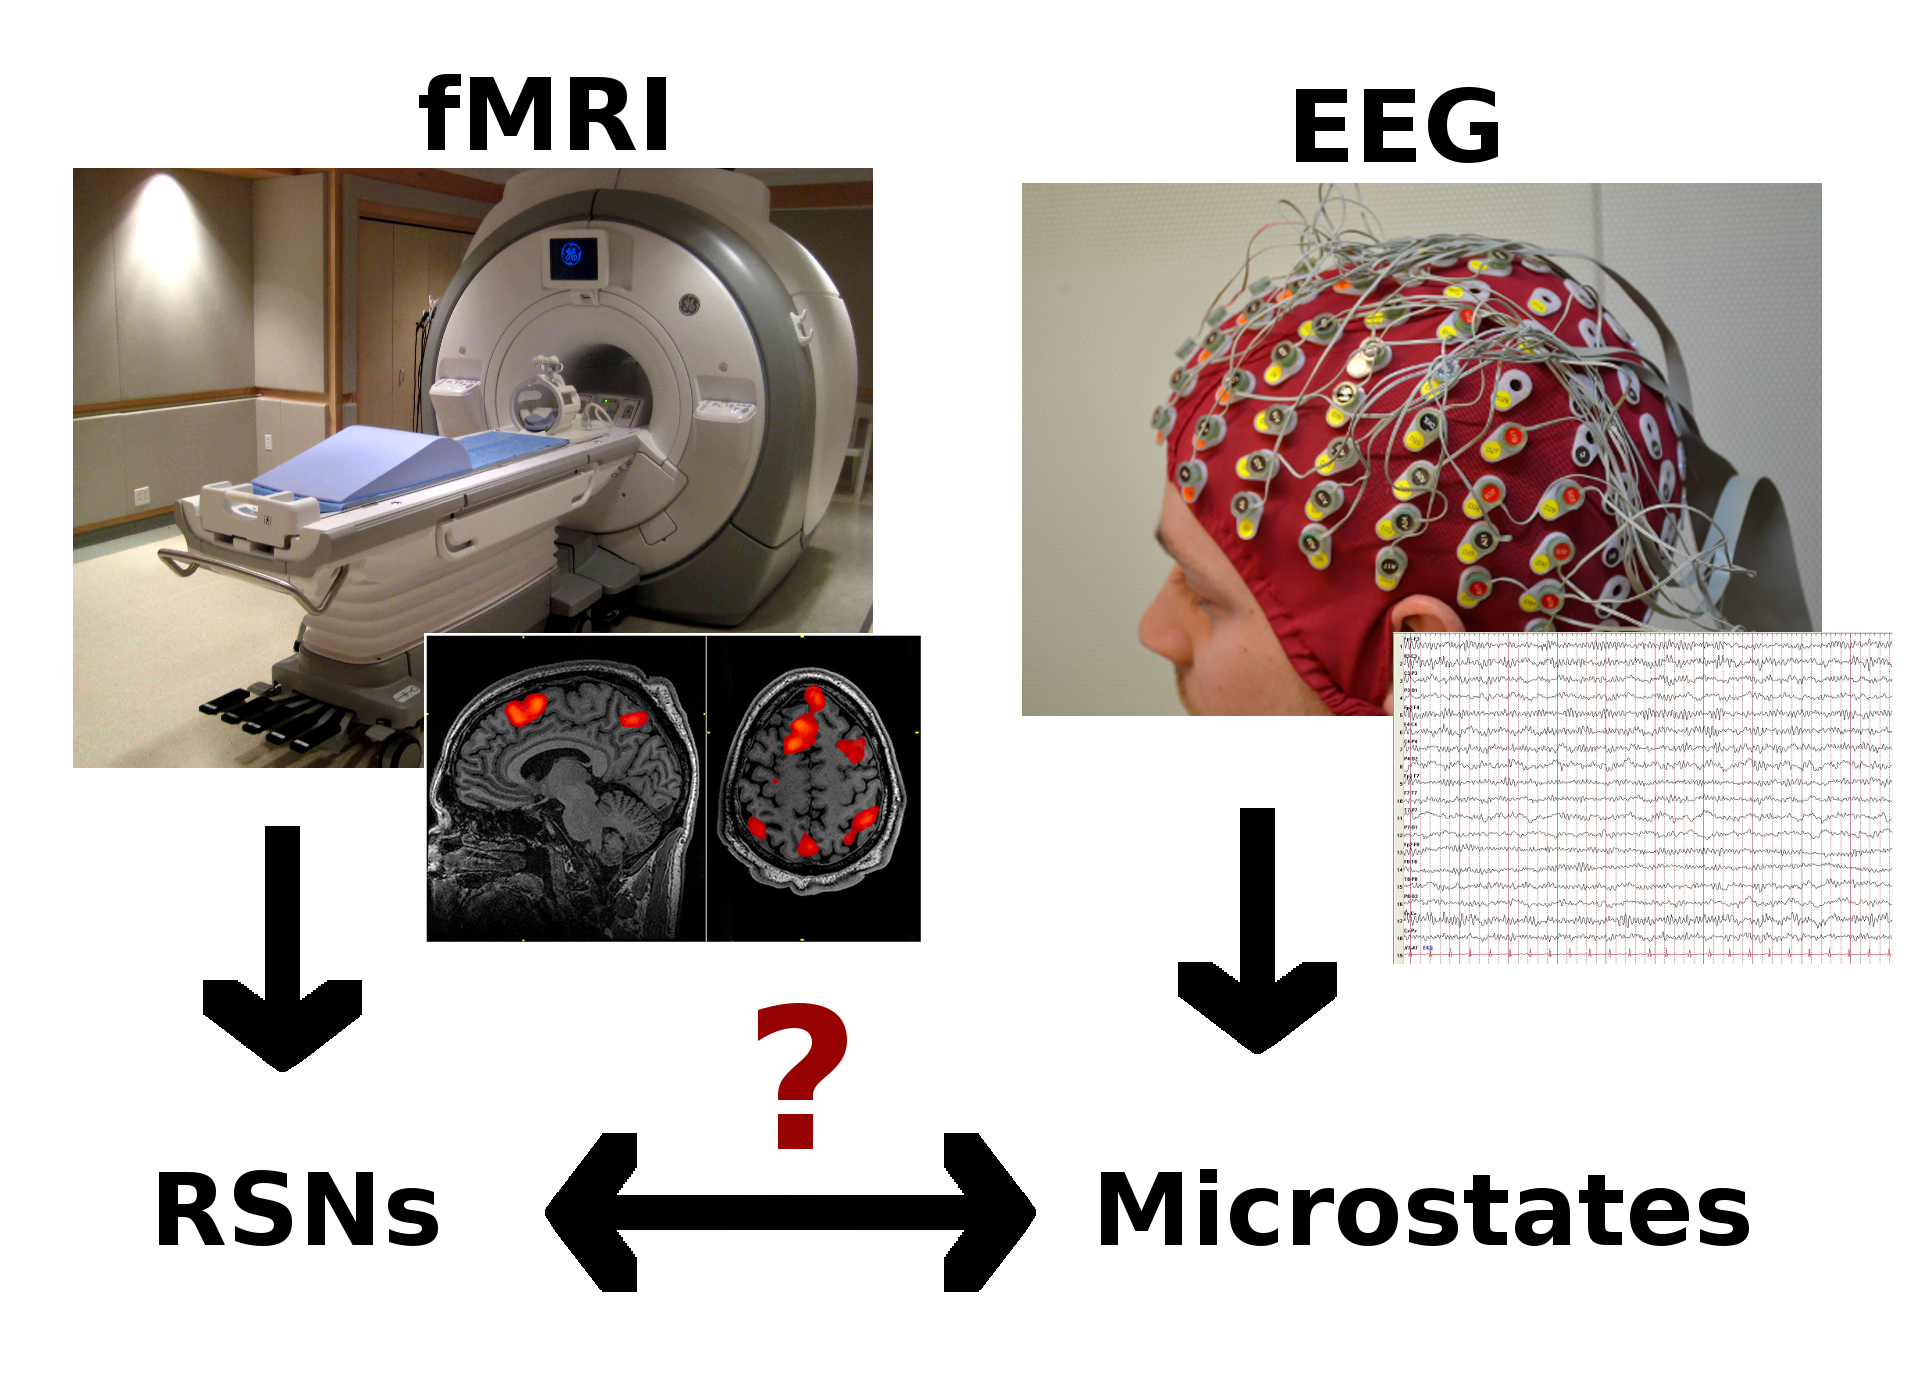
\includegraphics[scale=0.135]{fmri_eeg}
\end{center}
\end{figure} 

%\vspace{0.3cm}
%\begin{itemize}
%\item fMRI - Default Mode Network
%\vspace{0.3cm}
%\item EEG - Microstates
%\vspace{0.3cm}
%\item 
%\vspace{0.3cm}
%\item 
%\vspace{0.3cm}
%\item 
%\end{itemize}

\end{frame}


%% SLIDE 1
\begin{frame}[t]
\frametitle{Motivation - The Brain’s Dark Energy}
\framesubtitle{Default Mode Network - \cite{Raichle}}

\begin{columns}
    \begin{column}{0.48\textwidth}



\vspace{0.3cm}
\begin{itemize}
\item Energy consumption decreases only a few \% during rest
\vspace{0.3cm}
\item Why consume energy at rest
\vspace{0.3cm}
\item Resting State Networks\\
(Sensory/motor, visual etc.)
\vspace{0.3cm}
\item DMN - Most researched RSN
\end{itemize}
\begin{figure}[H]
\begin{center}
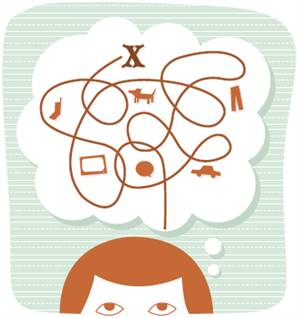
\includegraphics[scale=0.2]{wandering-mind}
\end{center}
\end{figure} 

    \end{column}
    \begin{column}{0.48\textwidth}

\begin{figure}[H]
\begin{center}
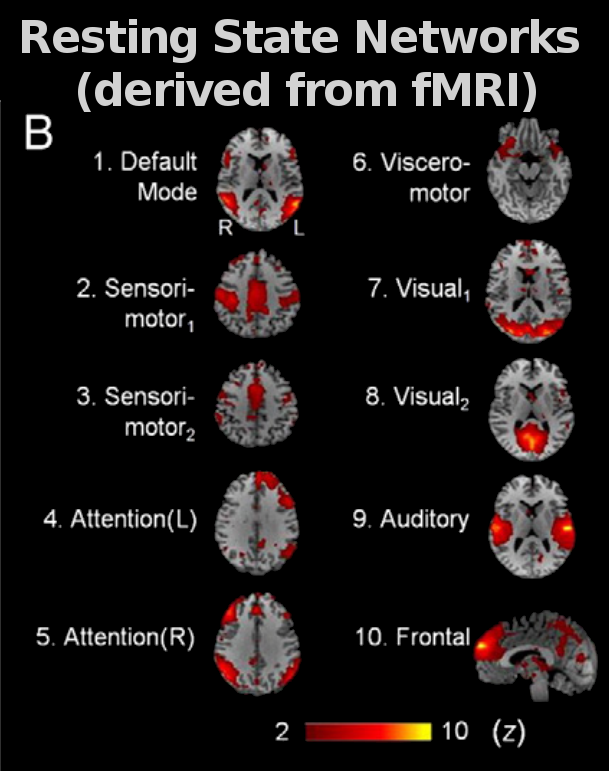
\includegraphics[scale=0.2]{RSNs}
\caption{Source: \cite{Yuan20122062}}
\end{center}
\end{figure}

    \end{column}
\end{columns}


\end{frame}


%%% SLIDE ?
\begin{frame}[t]
\frametitle{Microstates - The Atoms of Thought}
\framesubtitle{\cite{lehmann1980reference}}

\vspace{0.3cm}
\begin{itemize}
\item Transient quasi stable states ($\sim$100 ms)
\vspace{0.3cm}
\item Unique topographic distribution of the electrical field potential
\vspace{0.3cm}
\item Like the RSNs, the microstates are altered in a variety of brain disorders
\end{itemize}

\begin{figure}[H]
\begin{center}
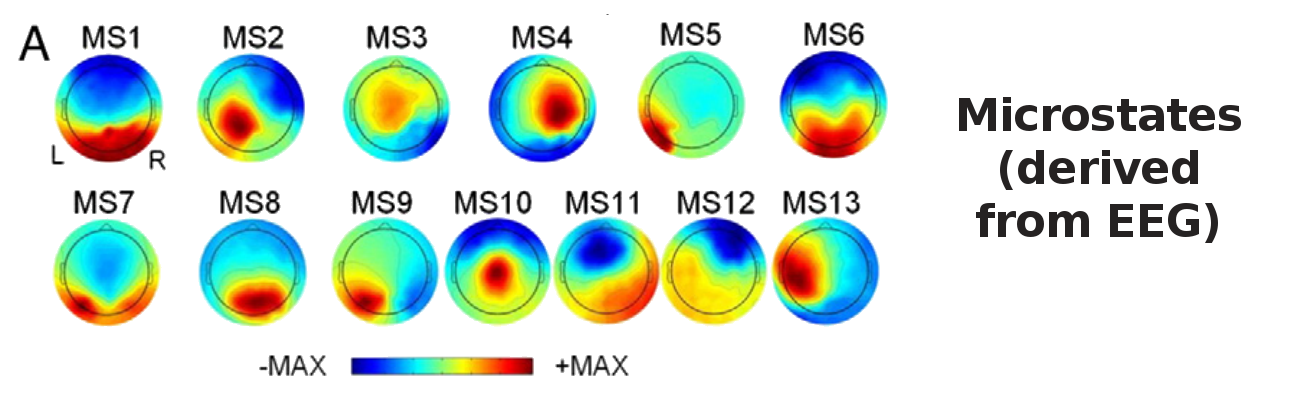
\includegraphics[scale=0.2]{microstates}
\caption{Source: \cite{Yuan20122062}}
\end{center}
\end{figure}

\end{frame}



%% SLIDE ?
\begin{frame}[t]
\frametitle{Data}
%\framesubtitle{}

\vspace{0.3cm}
\begin{itemize}
\item Simultaneous EEG and BOLD fMRI measurements of 20 patients recorded in Glostrup Hospital by Egil Rostrup and Ulrich Lindberg
\vspace{0.3cm}
\item 10 minutes brain activity from 30 diodes (EEG)
\vspace{0.3cm}
\item Default Mode Network ICA component of BOLD fMRI
\vspace{0.3cm}
\item Cleaned data
\vspace{0.3cm}
\item Artefacts still present (eye blink, heartbeat, movement etc.)
\end{itemize}

\end{frame}

%%% SLIDE ?
\begin{frame}[t]
\frametitle{Method and Plans}

\begin{enumerate}
\item Artifact removal in EEG data
\vspace{0.2cm}
\begin{itemize}
\item ICA, Spectrograms
\end{itemize}
\vspace{0.2cm}
\item Detecting Microstates
\vspace{0.3cm}
\begin{itemize}
\item Global Field Power
\vspace{0.3cm}
\item Temporal ICA
\end{itemize}

\vspace{0.3cm}
\item Predict DMN from microstates
\vspace{0.2cm}
\begin{itemize}
\item GLM (Regularized)
\vspace{0.3cm}
\item Gaussian process
\vspace{0.3cm}
\item Hemodynamic response function
\end{itemize}
\end{enumerate}

\end{frame}



\begin{frame}[plain,c]
%\frametitle{A first slide}

\begin{center}
\Huge Questions?
\end{center}

\end{frame}

%%% SLIDE ?
%\begin{frame}[t]
%	\frametitle{????}
%	%\framesubtitle{}
%	
%
%
%\end{frame}






\nocite{Yuan20122062}
\nocite{Raichle}
\nocite{lehmann1980reference}
\bibliographystyle{apalike} % press F11 in ordere to work
\bibliography{refs}
\end{document}